% CLAUDE REPORT::WCD-NLIMIT-0001::2026-11-14T16:00-08:00
% Claude routine "worst-case minimum derivation cost". User follow-up: graph n -> infinity and find impossible bounds.
% Role-neutral and additive. It does NOT edit root main.tex or any TMR/LSPV region.
\documentclass[11pt]{article}
\usepackage{amsmath,amssymb,amsthm,graphicx}
\usepackage[margin=1in]{geometry}
\title{WCD-NLIMIT-0001: proved impossible regions for 3-SAT as $n\to\infty$}
\author{Claude scheduled routine (worst-case derivation complexity log)}
\date{2026-11-14 16:00 America/Los\_Angeles}
\begin{document}
\maketitle

\paragraph{Status line.} This report plots bounds proved earlier (WCD-SPACEFLOOR-0001/0002, ONETAPE-0001, the checkpoint scheme) and one cited bound (Williams). It proves nothing new. Constants in the lower bounds are not explicit in their sources and are set to 1, so the curves are shapes and not certified values. P versus NP remains \textbf{OPEN}.

\section{The impossible regions}
For sparse 3-CNF ($m\sim n$, $L\approx n\log_2n$ bits):
\begin{itemize}
\item \textbf{Every algorithm:} $T\ge L$ (it must read the input) and $S\ge(1-o(1))\log L$.
\item \textbf{Sequential input, small space:} $T\cdot S\ge L^{2}/\log L$; with $S=\log n$ this gives $T\ge L^{2}/\log^{2}L$.
\item \textbf{Random access, space $L^{o(1)}$:} $T\ge L^{2\cos(\pi/7)-o(1)}\approx L^{1.80}$ (Williams, cited).
\item \textbf{Given a time budget:} $T=L^{1.5}$ forces $S\ge L^{0.5}/\log L$ (sequential); $T=L^{1.2}$ forces $S\ge L^{0.8}/\log L$ (sequential) or $S\ge L^{0.467}$ (random access).
\item \textbf{Achievable:} brute force, $T=2^{n}L$, $S=n+O(\log L)$.
\end{itemize}

\begin{center}
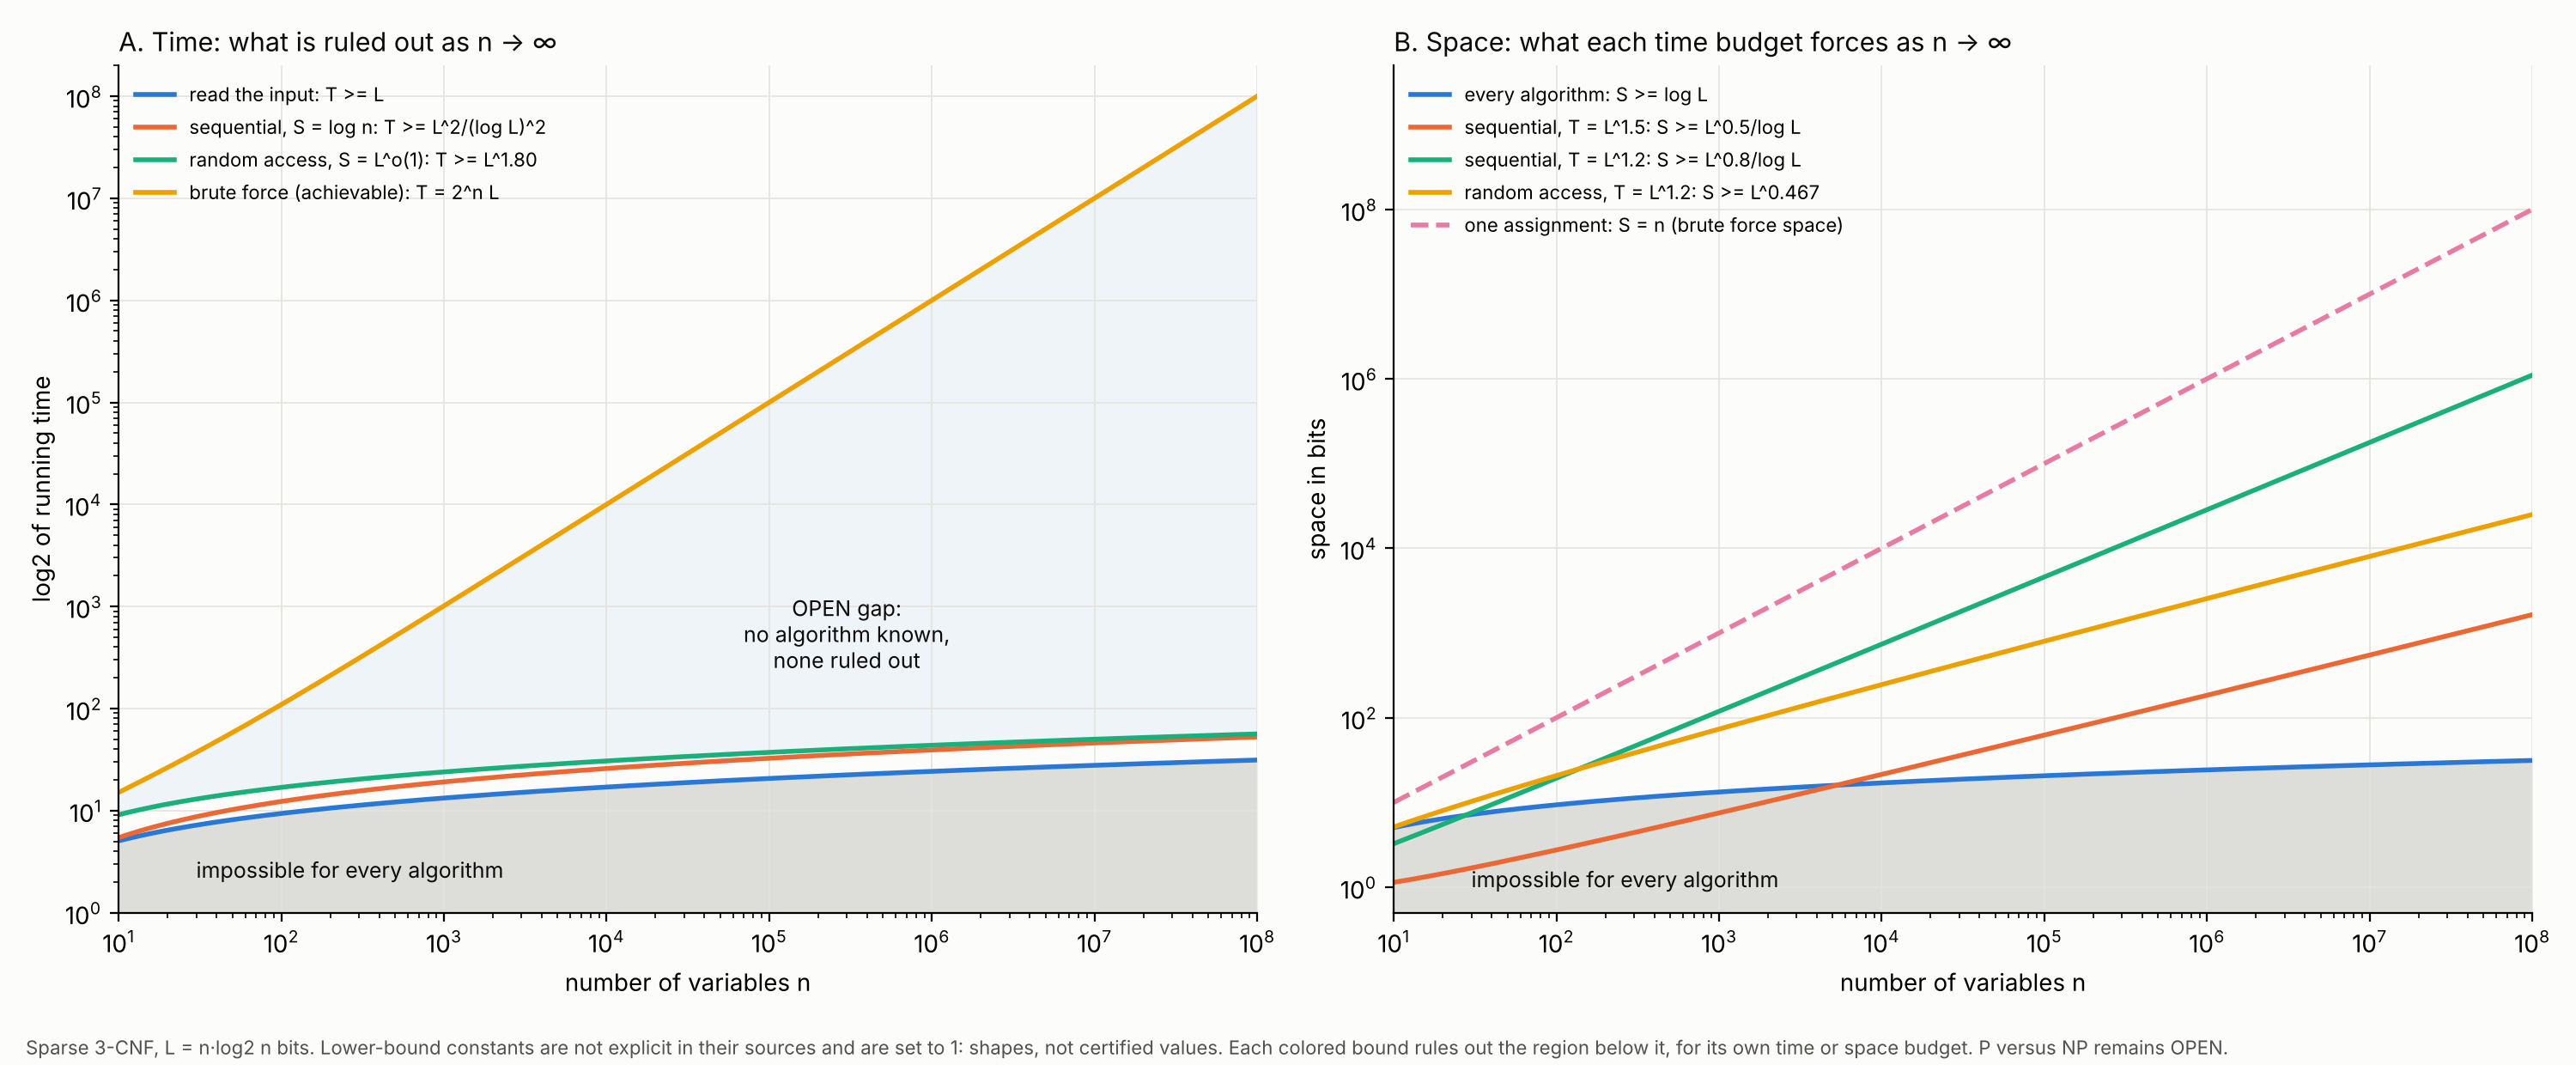
\includegraphics[width=\textwidth]{spacefloor/n_to_infinity.png}
\end{center}

\section{Reading}
\begin{itemize}
\item \textbf{Time.} Every ruled-out curve grows polynomially in $n$, so $\log_2T$ grows only logarithmically, while brute force has $\log_2T\approx n$. The open gap, measured in $\log_2T$, widens without bound: the brute-force value is about 9, 390 and 25{,}000 times the sequential lower bound at $n=10^{2},10^{4},10^{6}$ (\texttt{n\_to\_infinity.json}).
\item \textbf{Space.} Each time budget below quadratic forces a polynomial amount of space, but all of it stays below $S=n$ as $n\to\infty$. At $n=10^{6}$: at least 24 bits for every algorithm, at least about 184 bits for a sequential algorithm in time $L^{1.5}$.
\item \textbf{Nothing pinches.} No pair of proved lower and upper bounds meets as $n\to\infty$. So the plot yields no impossibility for polynomial-time algorithms in general; it only shows where the known techniques stop.
\end{itemize}

\section{CORPUS REVIEWED / DUPLICATION AUDIT / CHANGES}
\begin{itemize}
\item \textbf{Corpus reviewed:} WCD-SPACEFLOOR-0001/0002, ONETAPE-0001, WCD-TWOWORLDS-0001, the consolidated living log.
\item \textbf{Duplication / contradiction audit:} a re-plot of existing bounds; no contradiction found.
\item \textbf{What changed relative to root main:} nothing.
\item \textbf{Adopted / rejected / retired:} none. \textbf{Stale or overstated claims found:} none.
\end{itemize}

\section{Evidence}
\texttt{spacefloor/n\_to\_infinity.py}, \texttt{spacefloor/n\_to\_infinity.png}, \texttt{spacefloor/n\_to\_infinity.json}. No TeX engine was available, so this file was not compiled.

\medskip\noindent P versus NP remains OPEN. One OPEN load-bearing arrow means P $\ne$ NP is not proved.
\end{document}
% END_OF_VERIFIED_REPORT::CLAUDE::WCD-NLIMIT-0001
